Nella seguente tabella vengono riportati gli indici Gulpease\glo{} di tutti
i documenti prodotti finora.
    \rowcolors{2}{\evenRowColor}{\oddRowColor}
\renewcommand{\arraystretch}{1.5}
\begin{longtable}{ c c  C{4cm}  c  c }
    \caption{Tabella dell'indice di Gulpease RR} \\
    \rowcolor{\primaryColor}
    \textcolor{\secondaryColor}{
    \centering\textbf{Documento}}     & \textcolor{\secondaryColor}{\centering\textbf{Indice Gulpease}}    & \textcolor{\secondaryColor}
    {\centering\textbf{Esito}} \\
    \textit{Analisi dei Requisiti v1.0.0}           & 62                                    & Superato{} \\
    \textit{Glossario v1.0.0}                       & 72                                    & Superato{} \\
    \textit{Norme di Progetto v1.0.0}               & 68                                   & Superato{} \\
    \textit{Piano di Progetto v1.0.0}                & 64                                    & Superato{} \\
    \textit{Piano di Qualifica v1.0.0}                & 59                                    & Superato{} \\
    \textit{Studio di Fattibilità v1.0.0}               & 69                                    & Superato{} \\
    \textit{Verbale Interno 2020-10-31 v1.0.0}          & 72                                    & Superato{} \\
    \textit{Verbale Interno 2020-11-12 v1.0.0}          & 69                                    & Superato{} \\
    \textit{Verbale Interno 2020-12-11 v1.0.0}          & 73                                    & Superato{} \\
    \textit{Verbale Esterno 2020-12-18 v1.0.0}          & 76                                    & Superato{} \\
    \textit{Verbale Interno 2020-12-22 v1.0.0}          & 71                                    & Superato{} \\
    \textit{Verbale Interno 2021-01-05 v1.0.0}          & 74                                    & Superato{} \\
    \textit{Verbale Interno 2021-01-10 v1.0.0}          & 70                                    & Superato{} \\

\end{longtable}

\rowcolors{2}{\evenRowColor}{\oddRowColor}
\renewcommand{\arraystretch}{1.5}
\begin{longtable}{ c c  C{4cm}  c  c }
    \caption{Tabella dell'indice di Gulpease RP} \\
    \rowcolor{\primaryColor}
    \textcolor{\secondaryColor}{
    \centering\textbf{Documento}}     & \textcolor{\secondaryColor}{\centering\textbf{Indice Gulpease}}    & \textcolor{\secondaryColor}
    {\centering\textbf{Esito}} \\
    \textit{Analisi dei Requisiti v2.0.0}           & 70                                    & Superato{} \\
    \textit{Glossario v2.0.0}                       & 73                                    & Superato{} \\
    \textit{Norme di Progetto v2.0.0}               & 72                                   & Superato{} \\
    \textit{Piano di Progetto v2.0.0}                & 65                                    & Superato{} \\
    \textit{Piano di Qualifica v2.0.0}                & 68                                    & Superato{} \\
    \textit{Verbale Esterno 2021-01-22 v1.0.0}          & 71                                    & Superato{} \\
    \textit{Verbale Interno 2020-01-29 v1.0.0}          & 69                                    & Superato{} \\
    \textit{Verbale Interno 2020-02-10 v1.0.0}          & 73                                    & Superato{} \\
    \textit{Verbale Esterno 2020-02-18 v1.0.0}          & 68                                    & Superato{} \\
    \textit{Verbale Interno 2020-02-25 v1.0.0}          & 70                                    & Superato{} \\
    \textit{Verbale Interno 2020-03-06 v1.0.0}          & 67                                    & Superato{} \\
\end{longtable}

\begin{figure}[H]
	\centering
	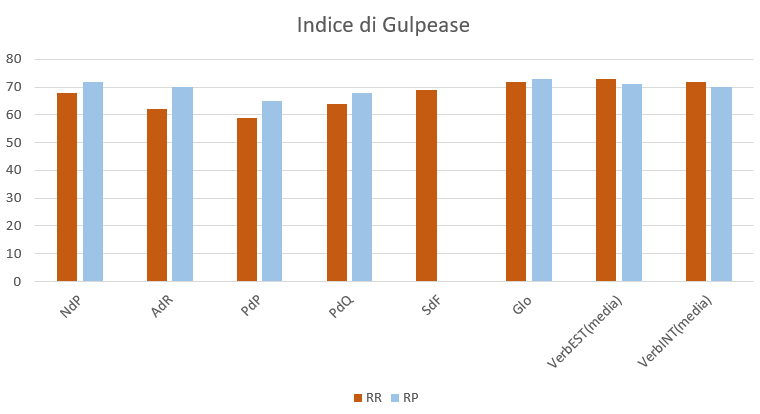
\includegraphics[scale=0.8]{src/ResocontoVerifica/src/img/indiceGulpease.png}
	\caption{Indice di Gulpease}
\end{figure}

